\subsection{Protocol} \label{protocol}
The protocol of the experiment contains 16 slides plus one slide for the welcoming and two slides for thanking the
experimentee and saying goodbye. The slides are changing after every performed gesture. A gesture can be performed by
pressing the \textit{B} button, moving the controller and releasing the \textit{B} button after the gesture. As
mentioned in section \ref{experiment} does the experiment consists of two parts, the recording of 8 test gestures and
the repetition of those gestures mixed with physical activities. All slides of the experiment are shown in
figure~\ref{fig:slides}.

\begin{figure}[H]
    \begin{center}
        \begin{tabular}{cccc}
            \frame{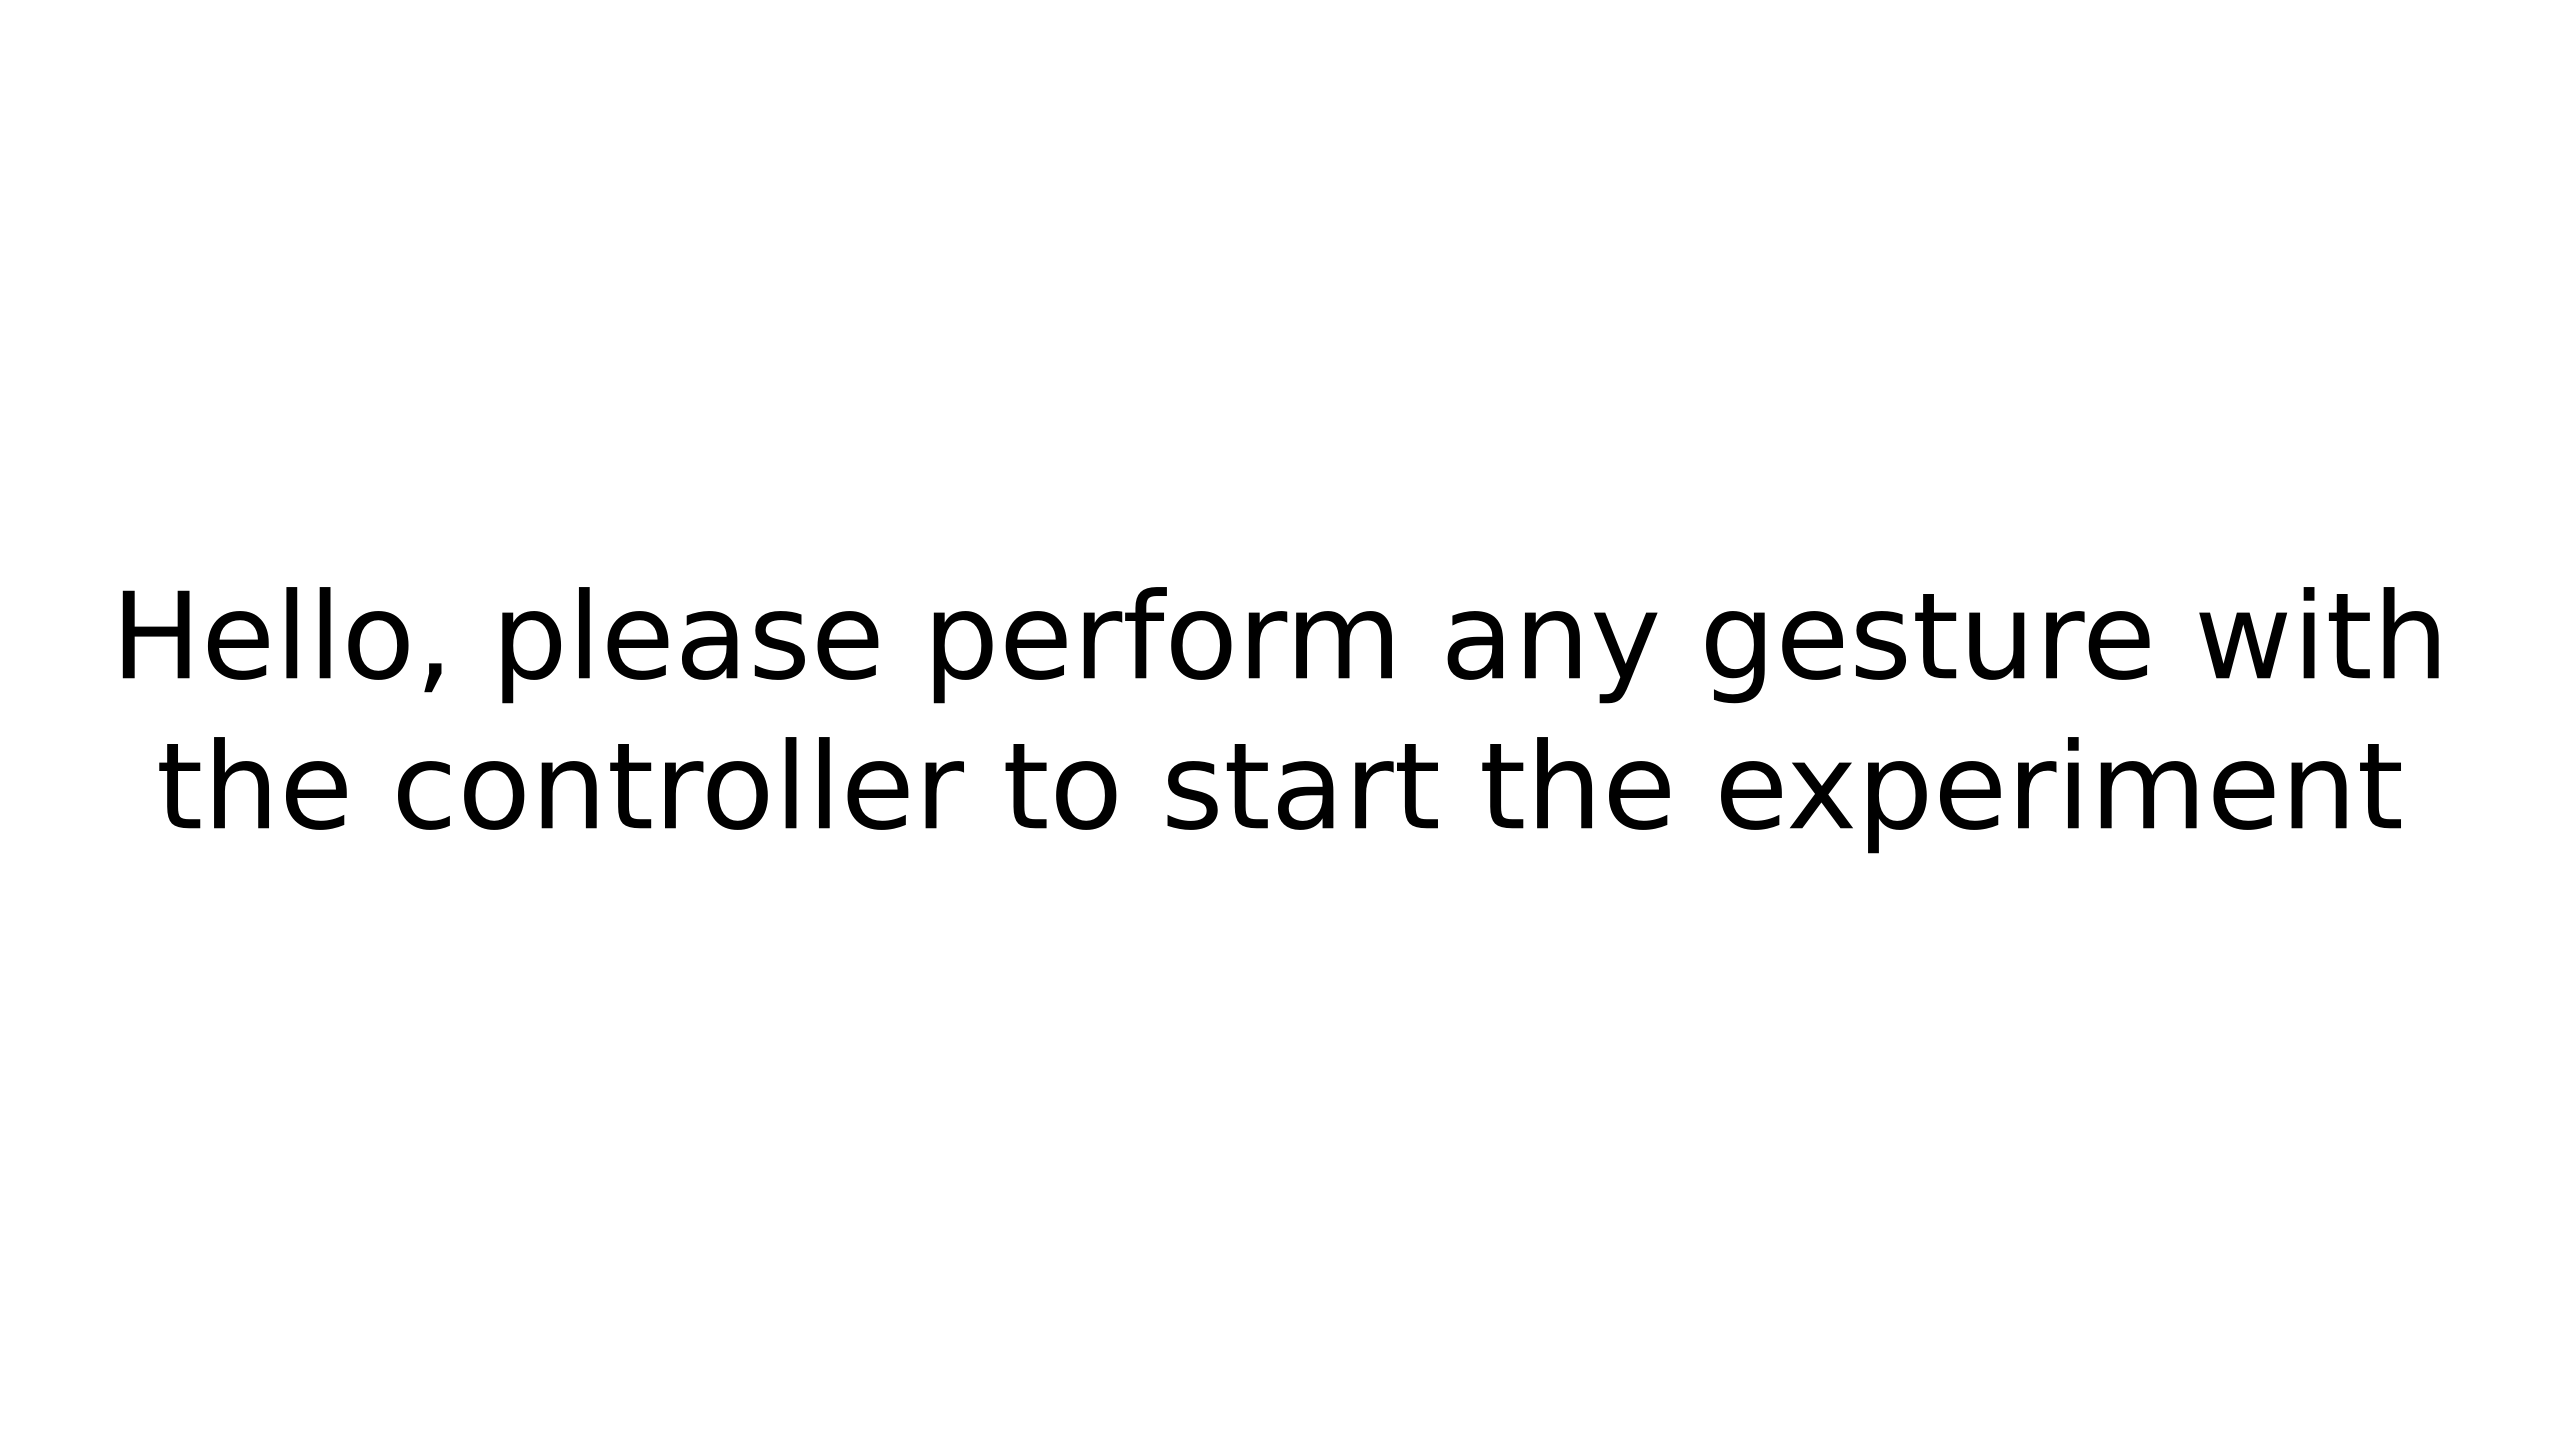
\includegraphics[width=0.24\textwidth]{1.png}} &
            \frame{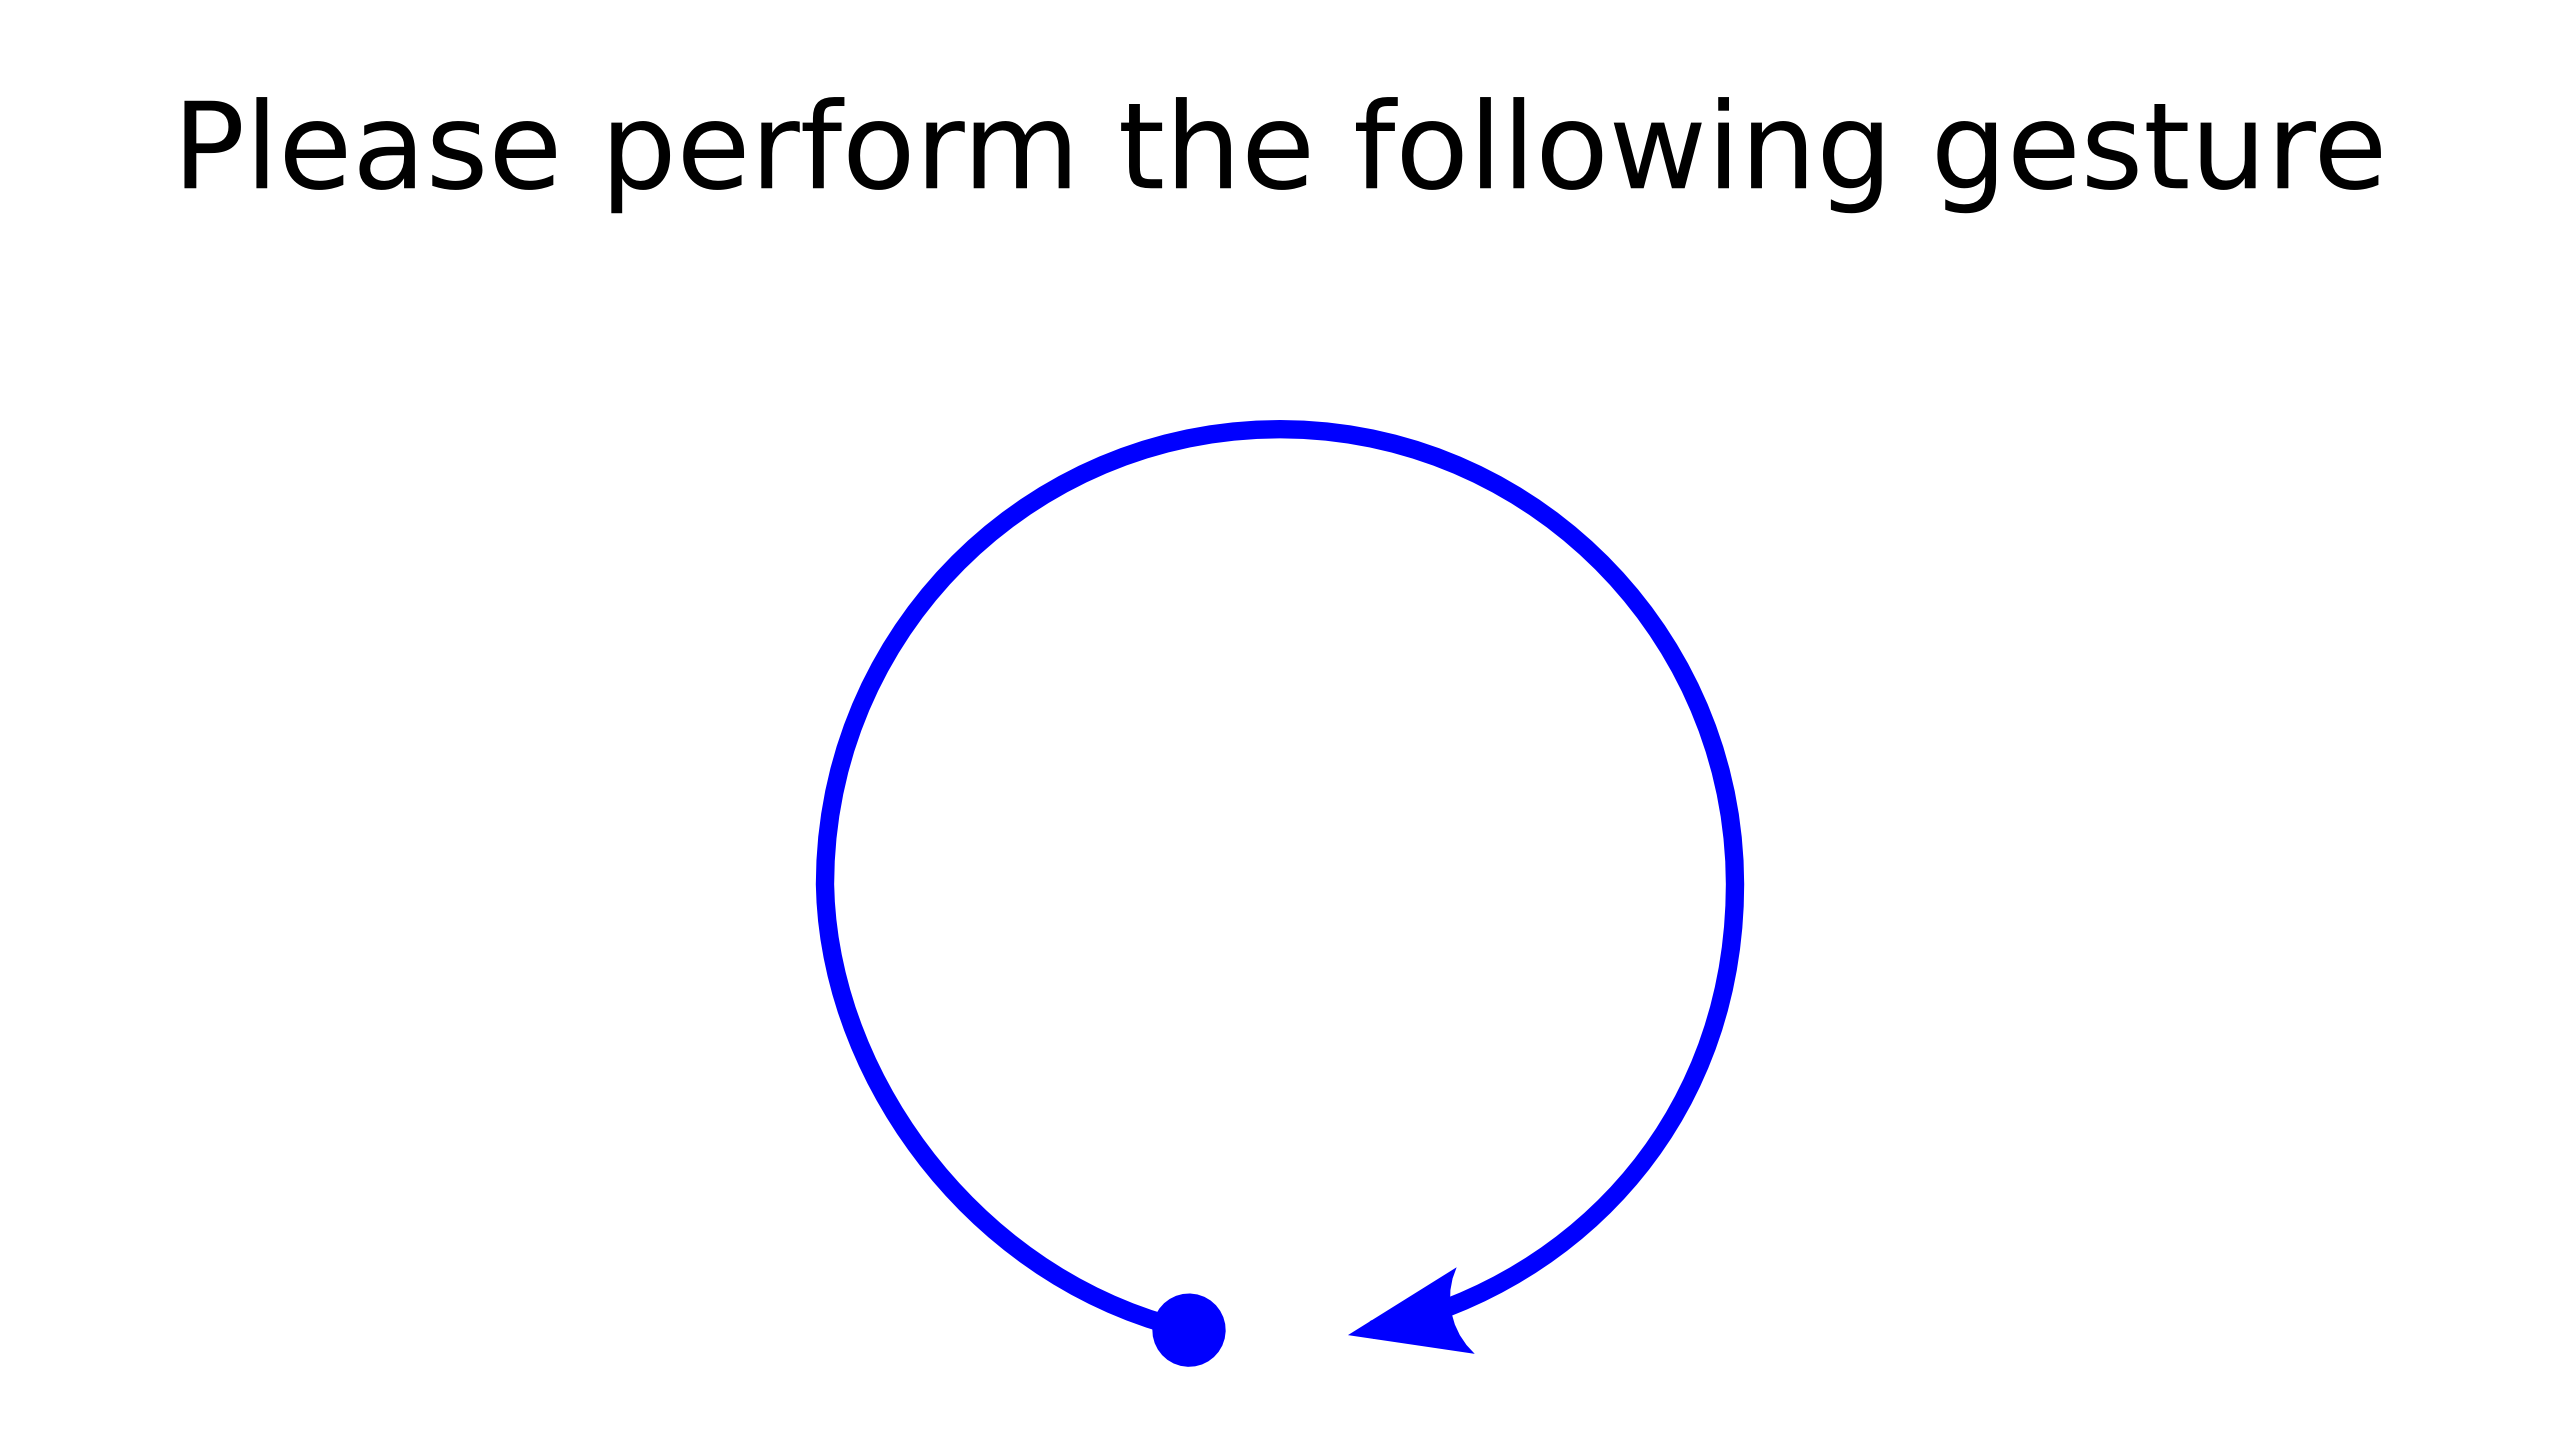
\includegraphics[width=0.24\textwidth]{2.png}} &
            \frame{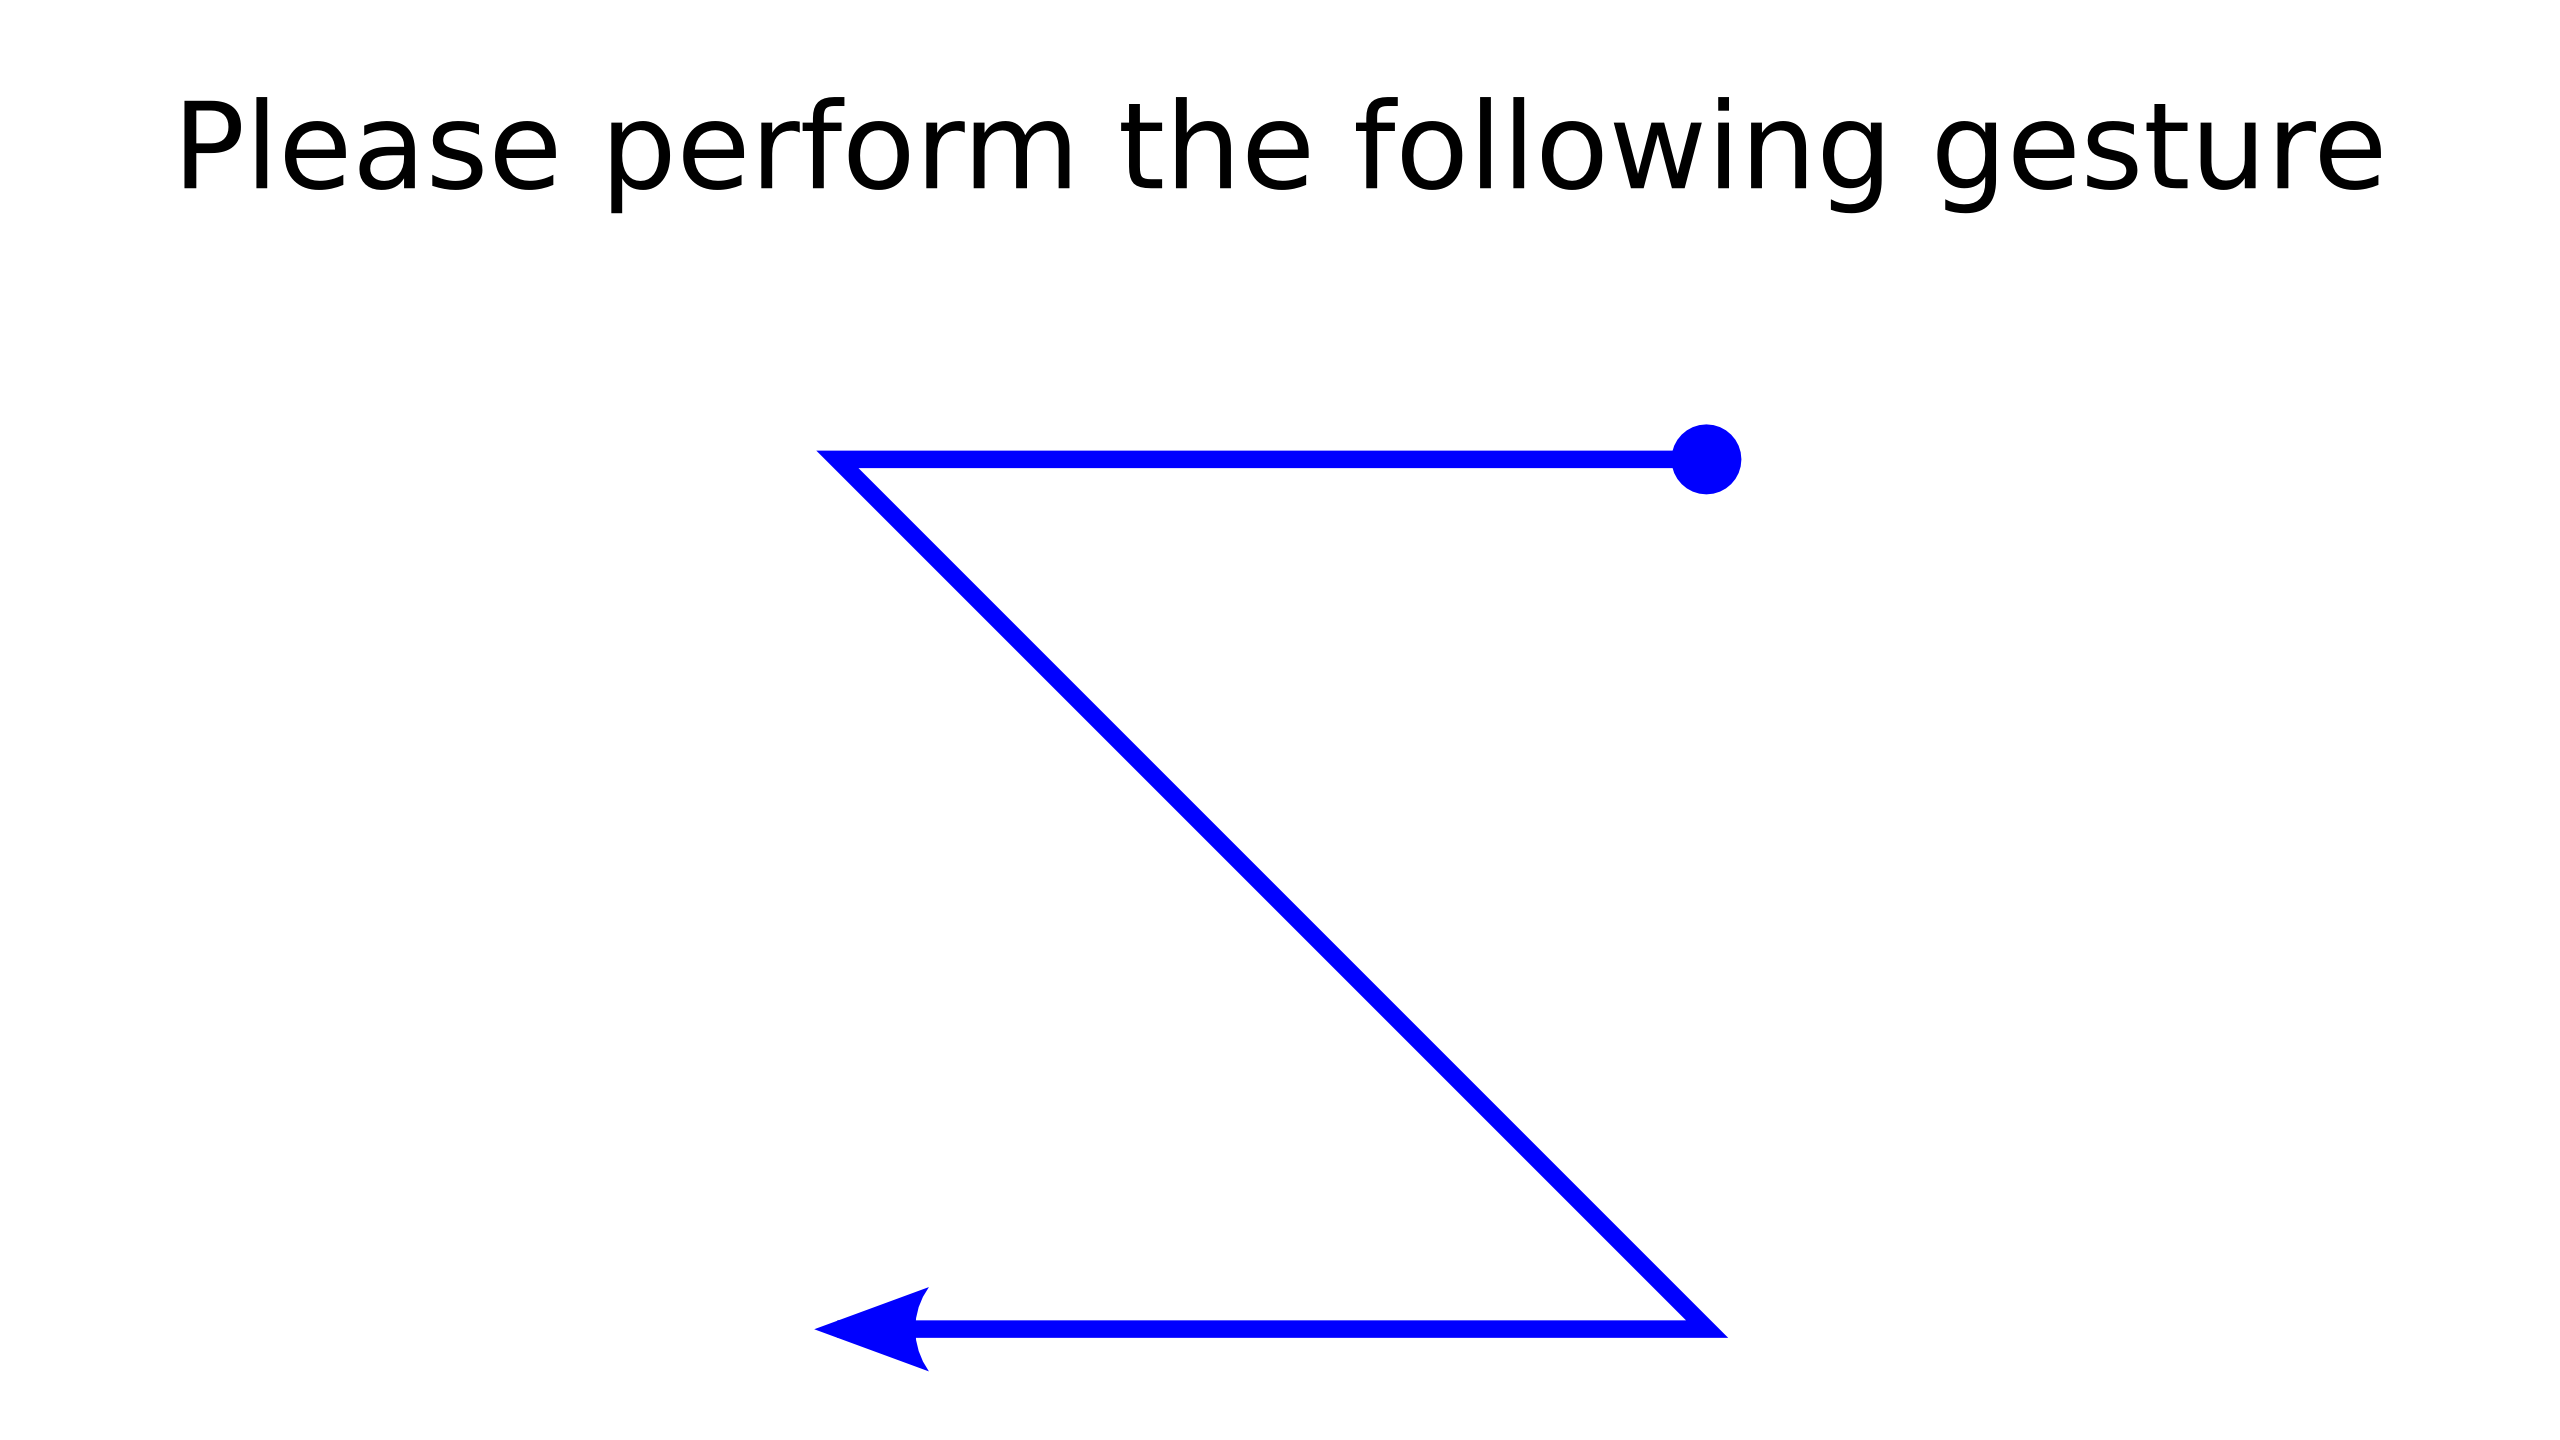
\includegraphics[width=0.24\textwidth]{3.png}} &
            \frame{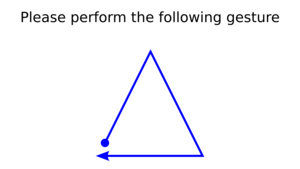
\includegraphics[width=0.24\textwidth]{4.png}} \\
            (a) \vspace{0.5ex} & (b) \vspace{0.5ex} & (c) \vspace{0.5ex} & (d) \vspace{0.5ex} \\
            \frame{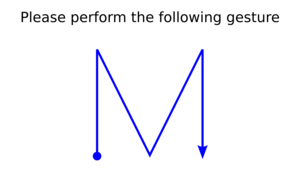
\includegraphics[width=0.24\textwidth]{5.png}} &
            \frame{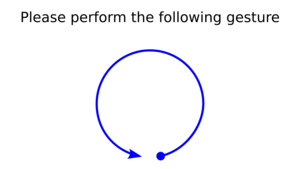
\includegraphics[width=0.24\textwidth]{6.png}} &
            \frame{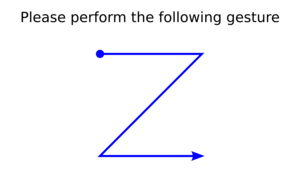
\includegraphics[width=0.24\textwidth]{7.png}} &
            \frame{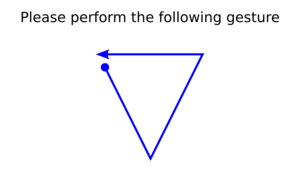
\includegraphics[width=0.24\textwidth]{8.png}} \\
            (e) \vspace{0.5ex} & (f) \vspace{0.5ex} & (g) \vspace{0.5ex} & (h) \vspace{0.5ex} \\
            \frame{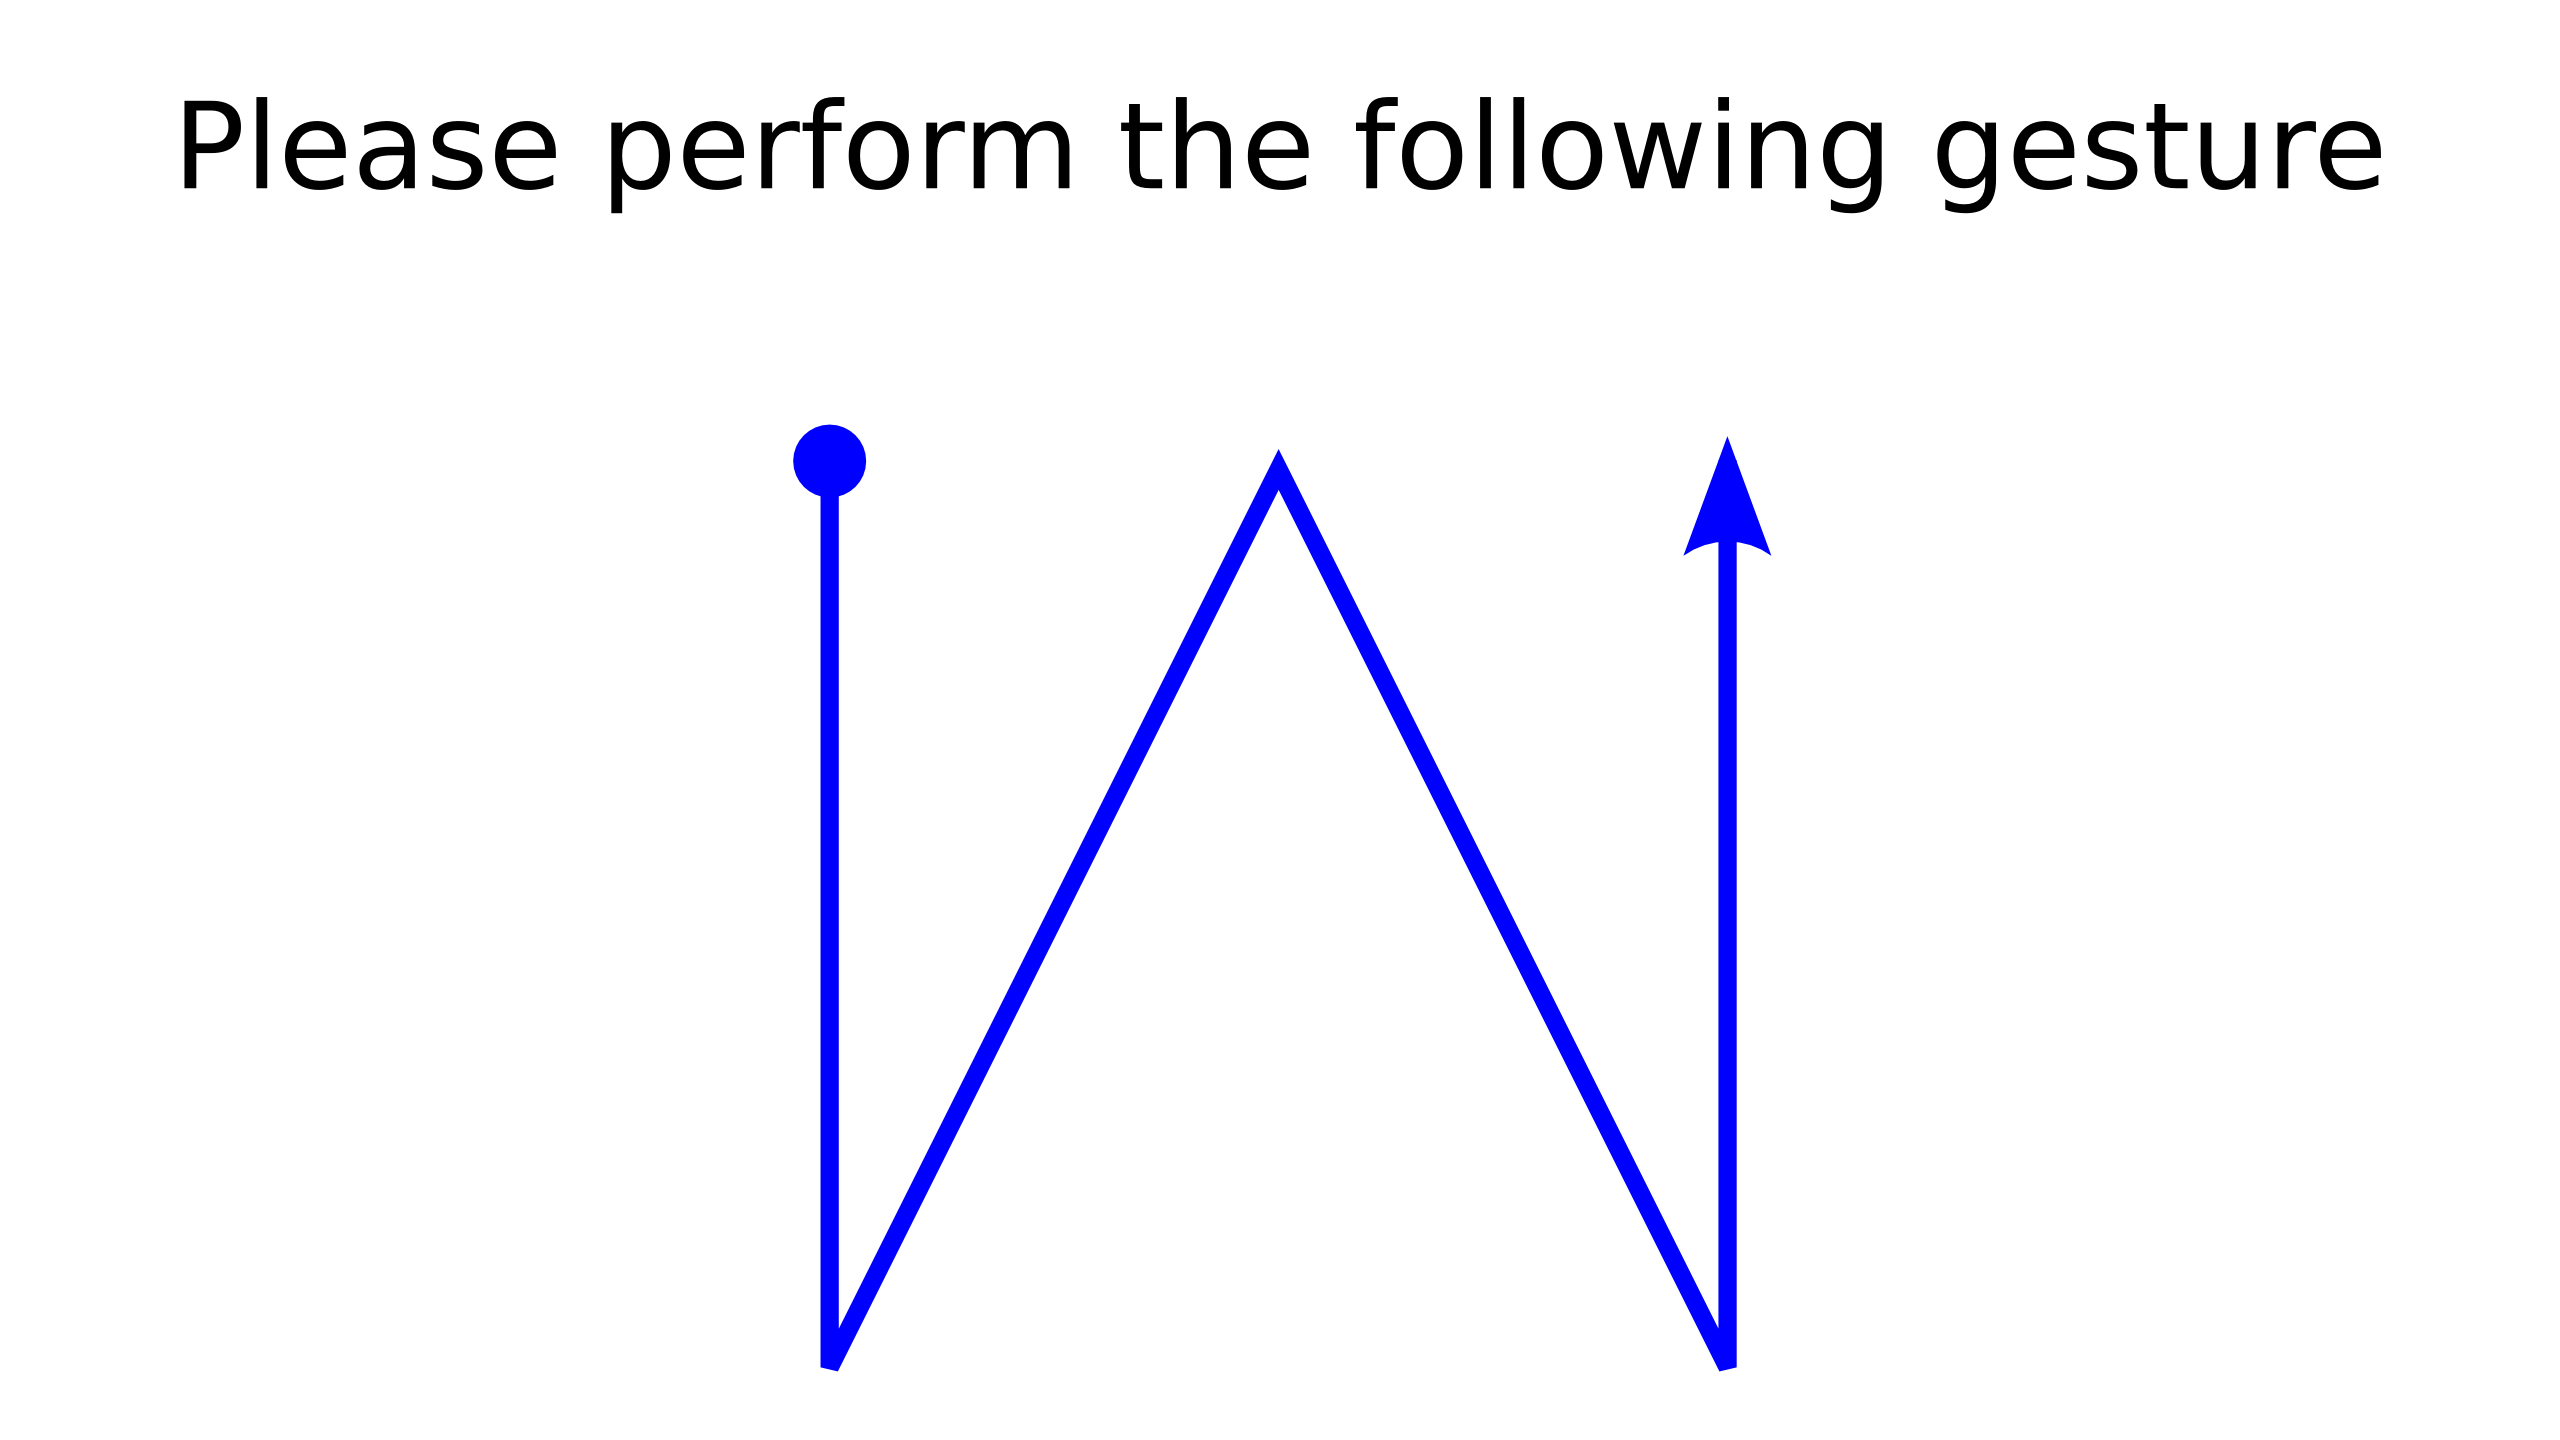
\includegraphics[width=0.24\textwidth]{9.png}} &
            \frame{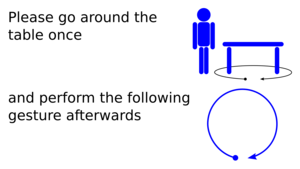
\includegraphics[width=0.24\textwidth]{10.png}} &
            \frame{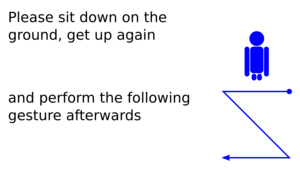
\includegraphics[width=0.24\textwidth]{11.png}} &
            \frame{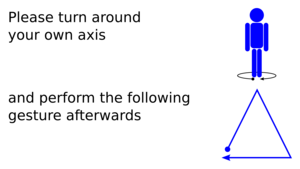
\includegraphics[width=0.24\textwidth]{12.png}} \\
            (i) \vspace{0.5ex} & (j) \vspace{0.5ex} & (k) \vspace{0.5ex} & (l) \vspace{0.5ex} \\
            \frame{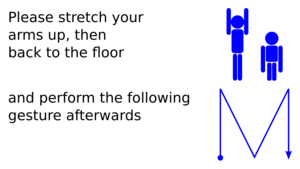
\includegraphics[width=0.24\textwidth]{13.png}} &
            \frame{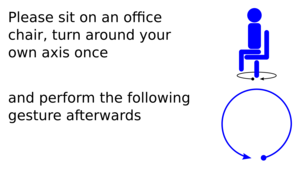
\includegraphics[width=0.24\textwidth]{14.png}} &
            \frame{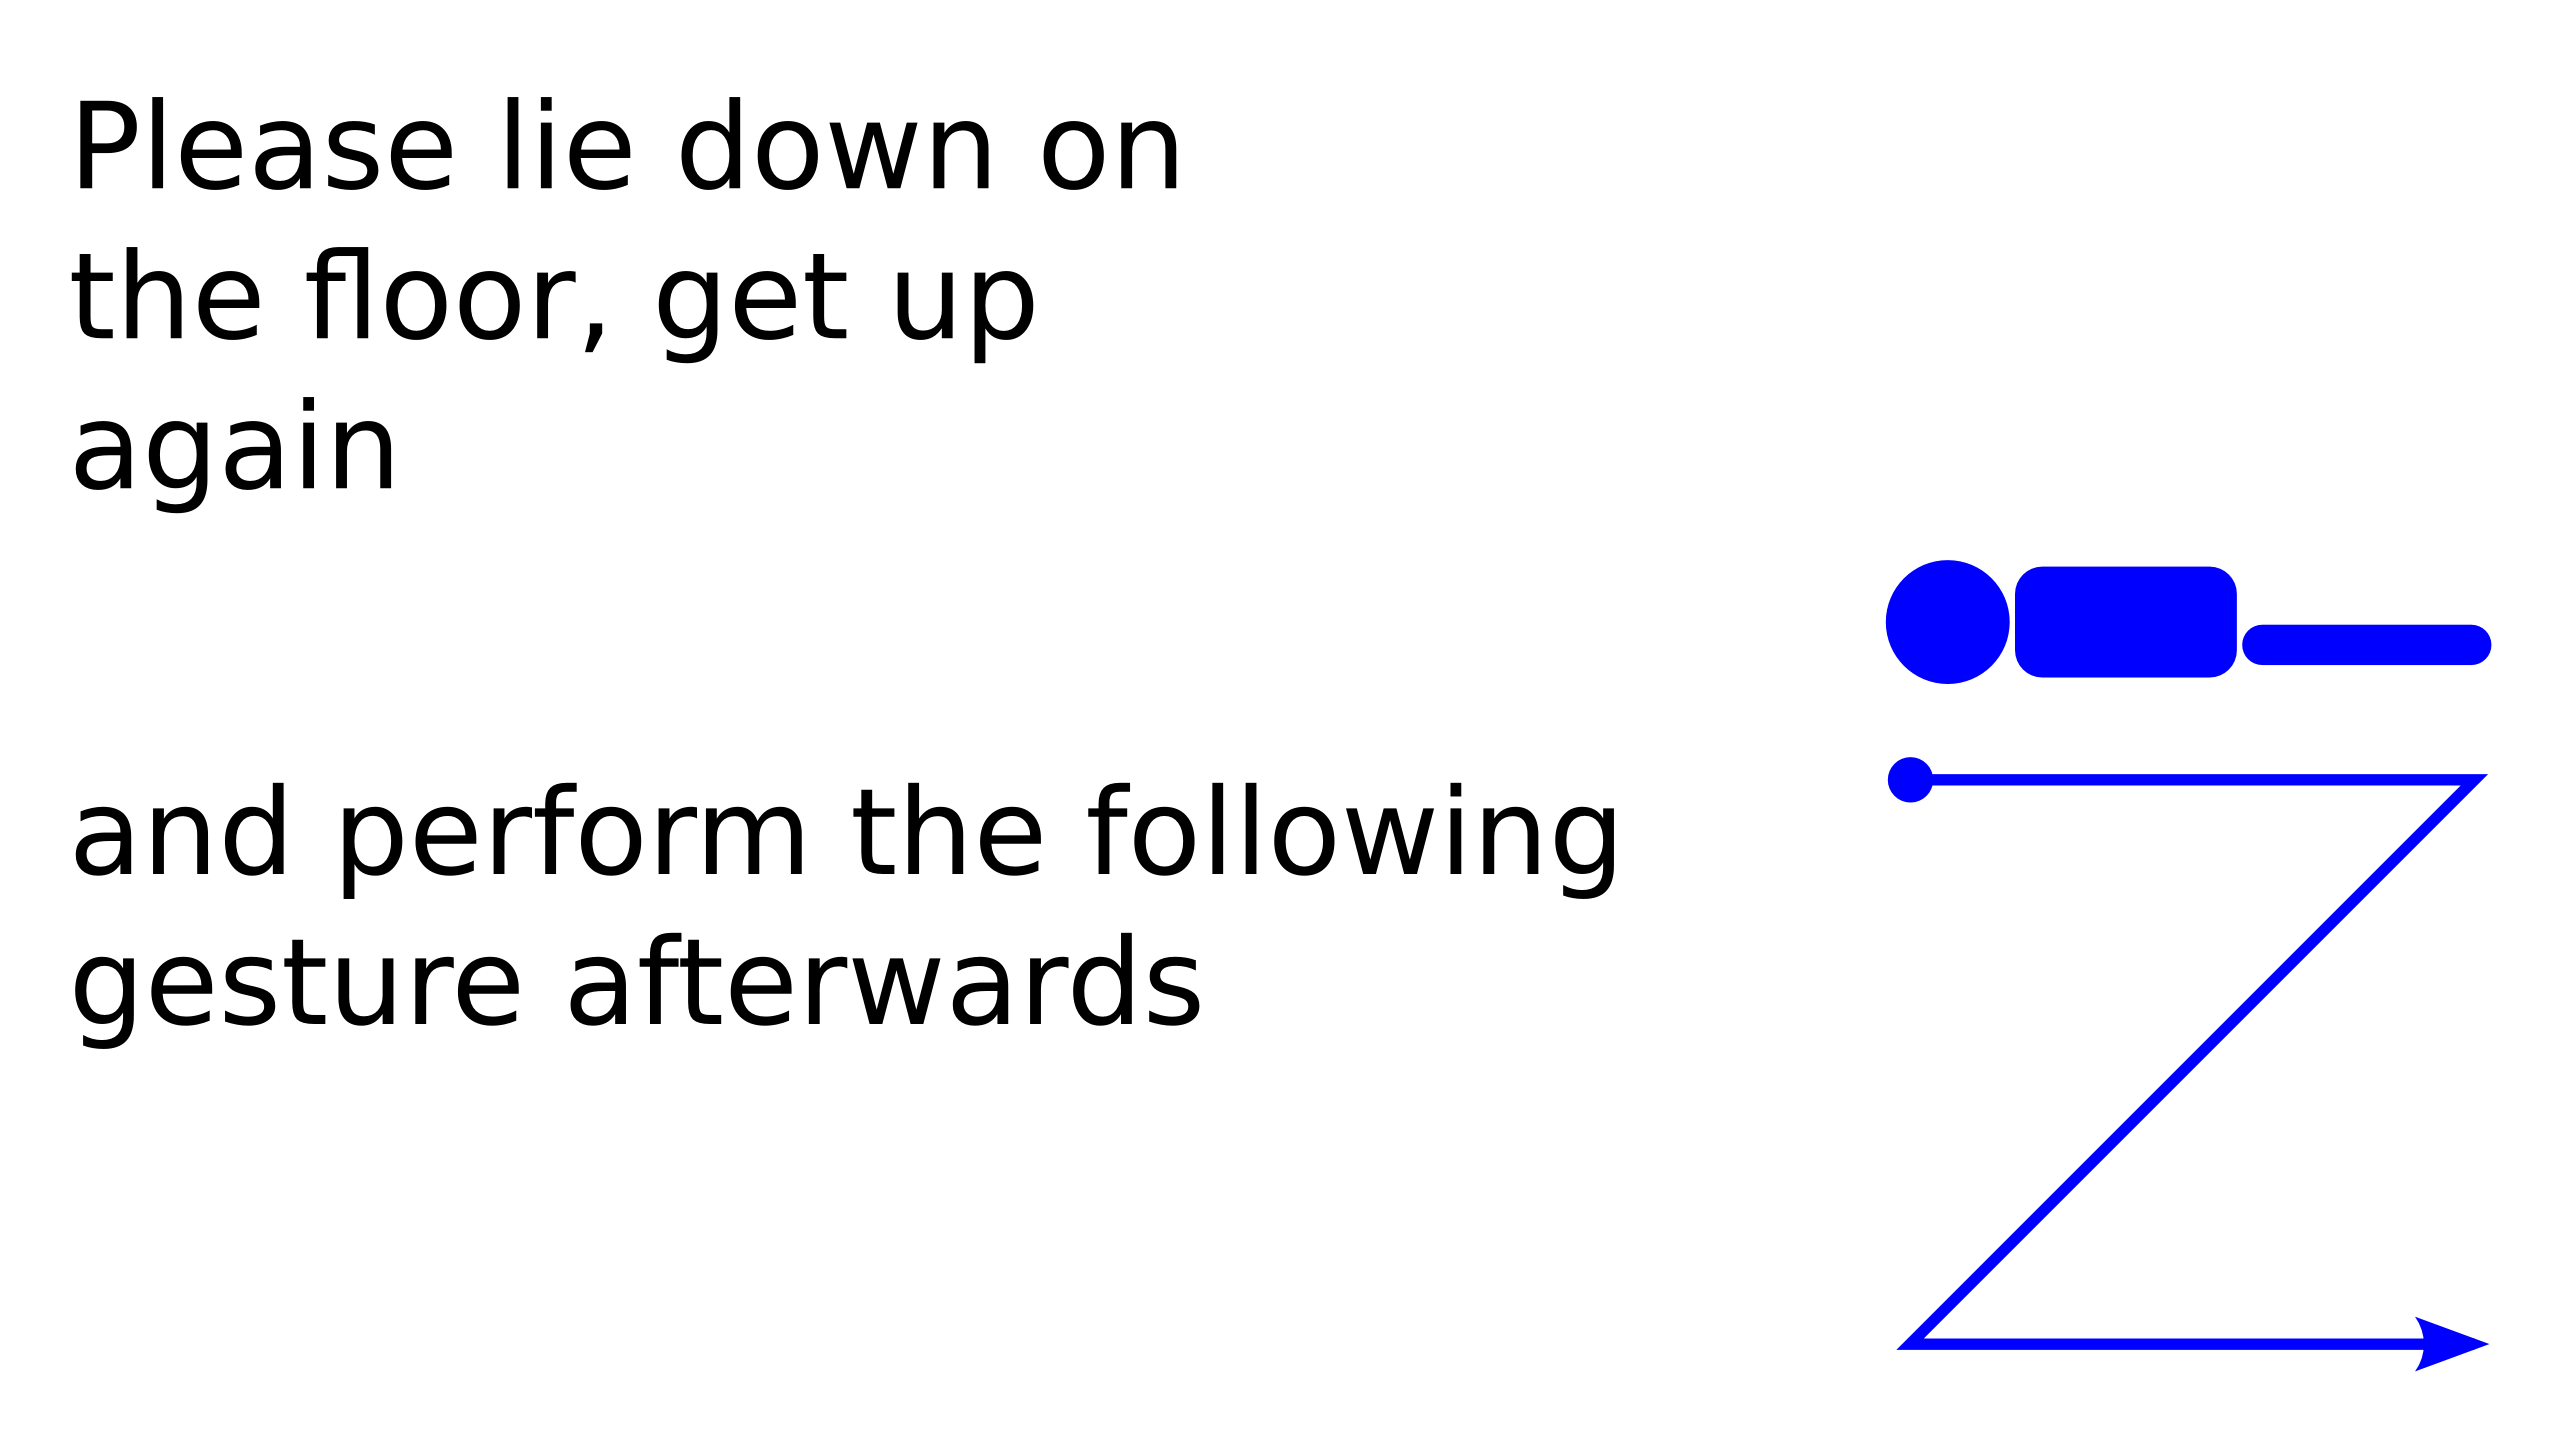
\includegraphics[width=0.24\textwidth]{15.png}} &
            \frame{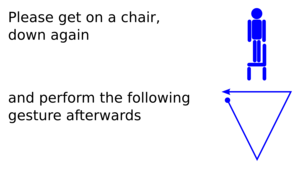
\includegraphics[width=0.24\textwidth]{16.png}} \\
            (m) \vspace{0.5ex} & (n) \vspace{0.5ex} & (o) \vspace{0.5ex} & (p) \vspace{0.5ex} \\
            \frame{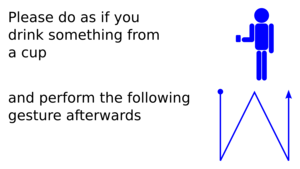
\includegraphics[width=0.24\textwidth]{17.png}} &
            \frame{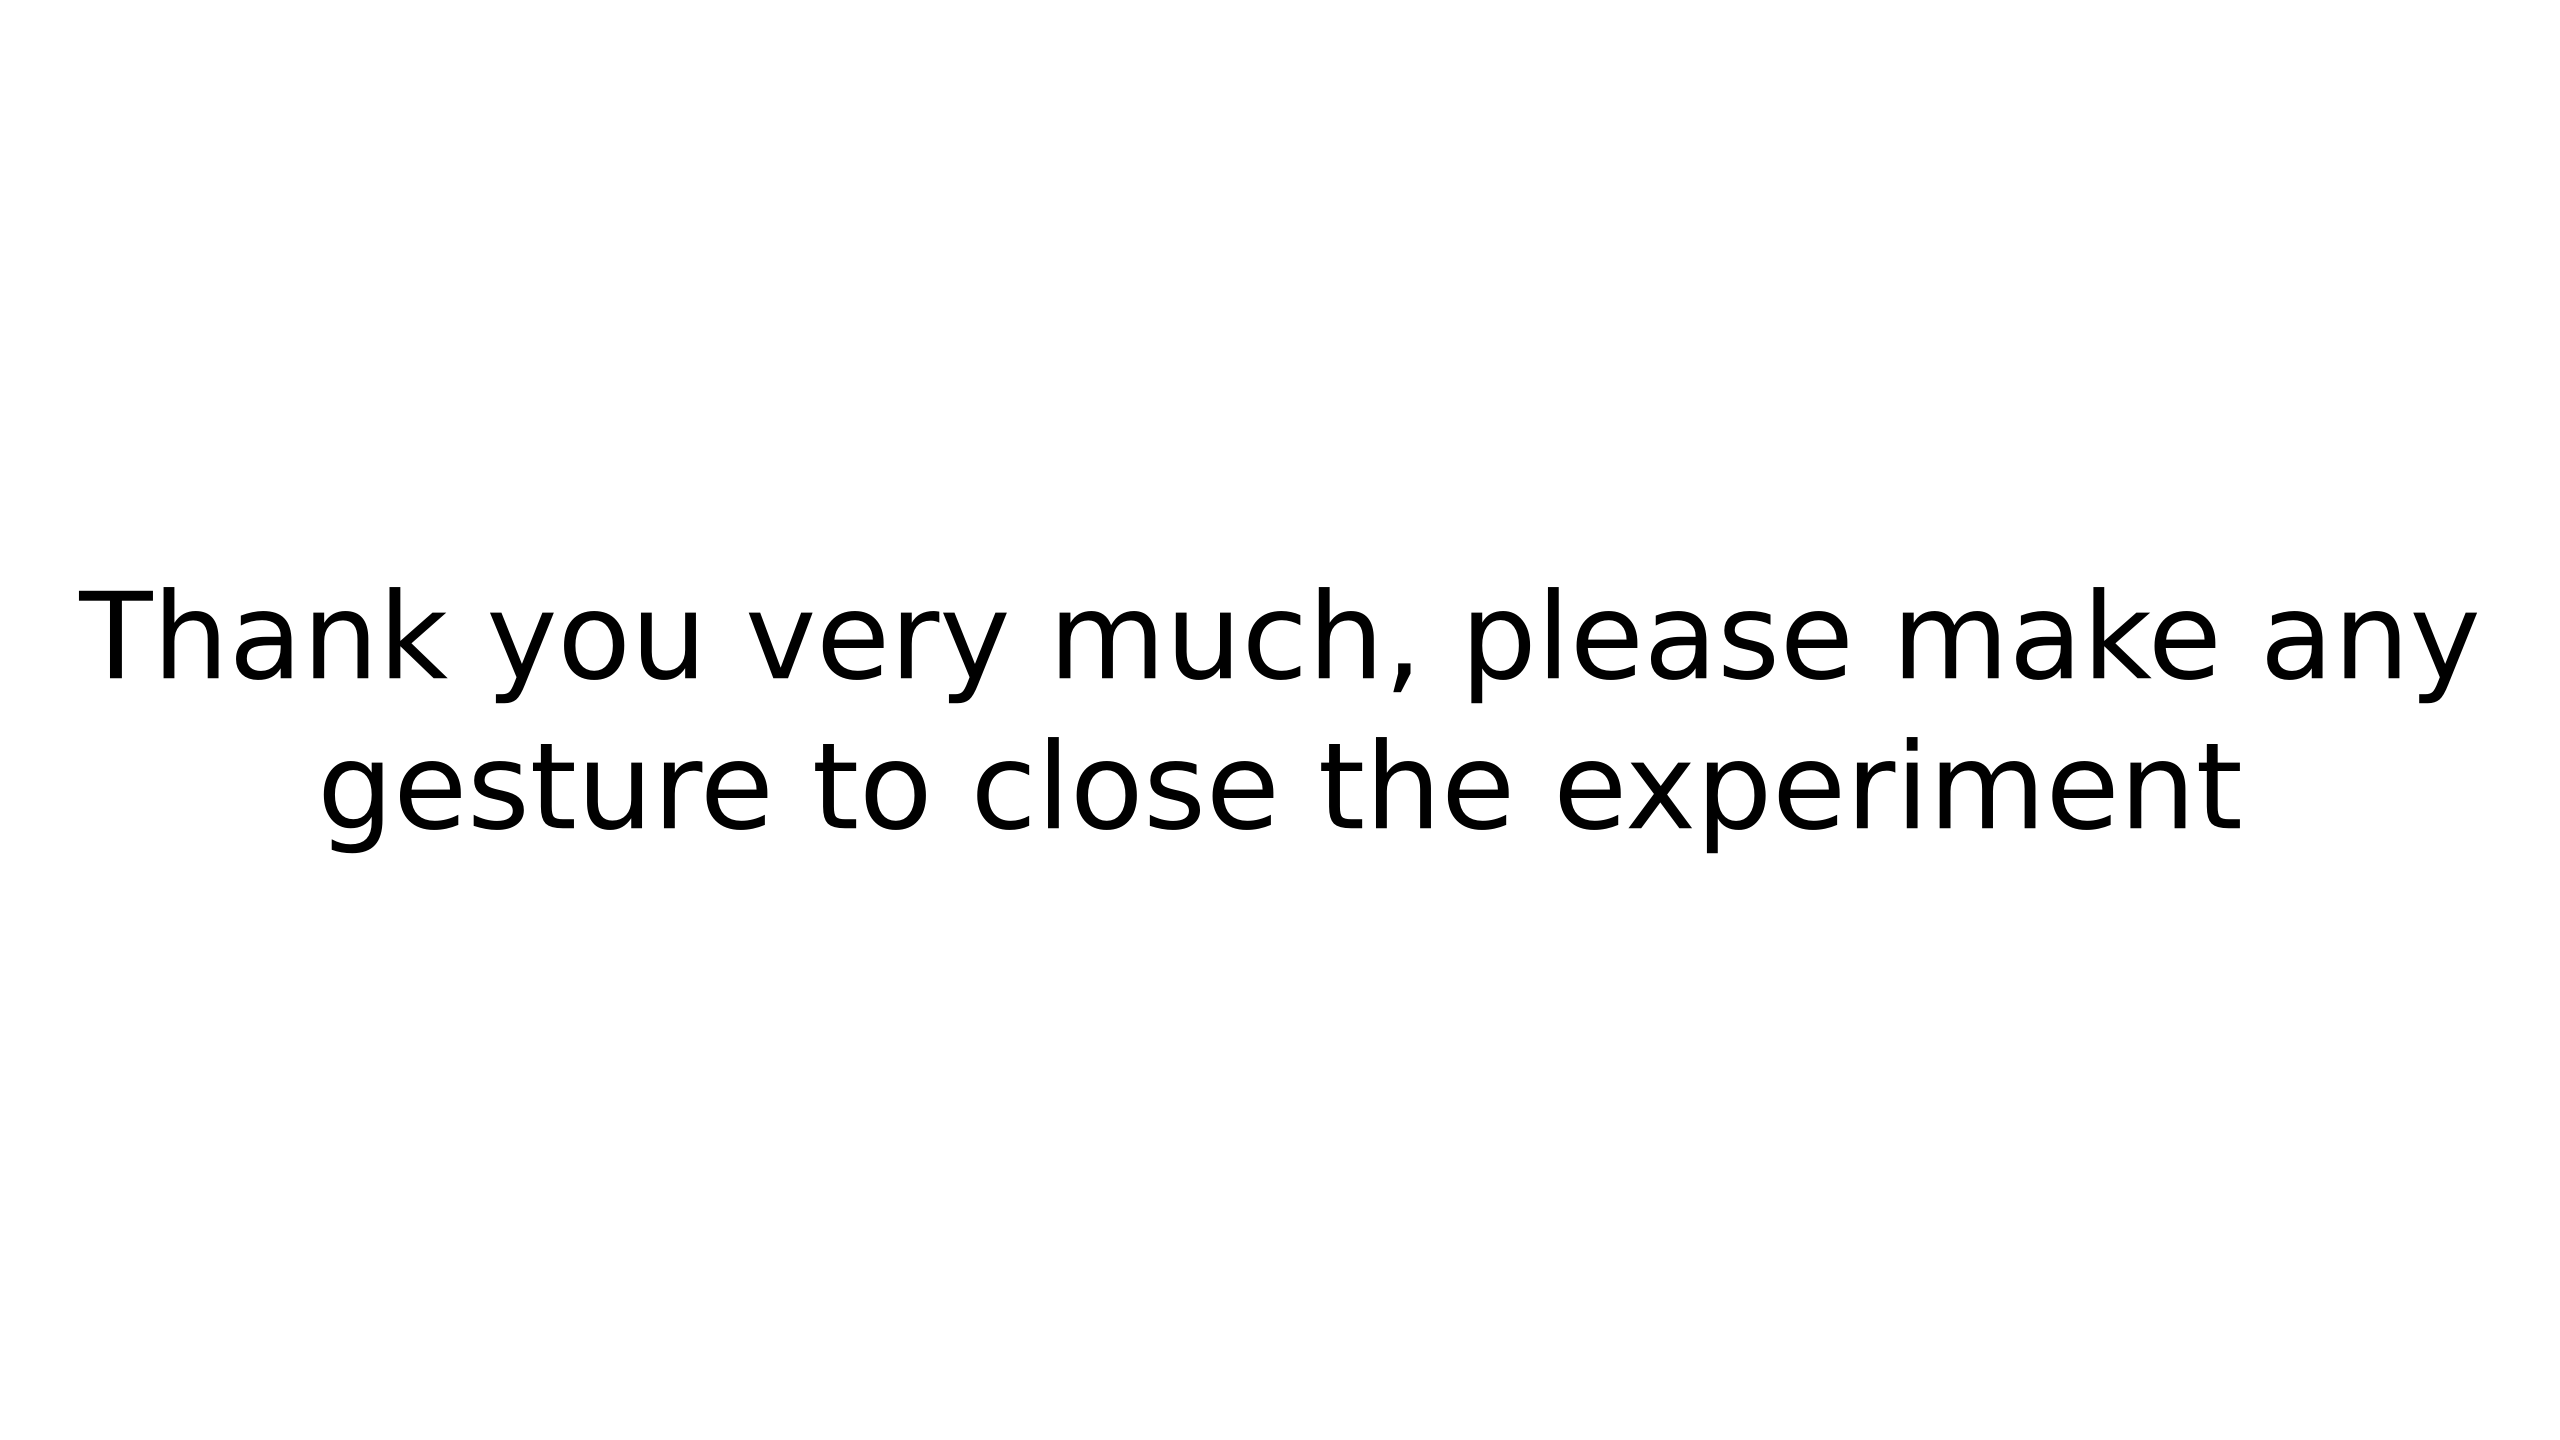
\includegraphics[width=0.24\textwidth]{18.png}} &
            \frame{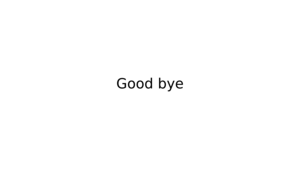
\includegraphics[width=0.24\textwidth]{19.png}} & \\
            (q) & (r) & (s) & \\
        \end{tabular}
    \end{center}
    \caption{The slides that are guiding the experimentees.}
    \label{fig:slides}
\end{figure}

Slide (a) of figure \ref{fig:slides} has the task to welcome the experimentee and is later used in evaluation to mark
the start of the recording. The slides (b) to (i) of figure \ref{fig:slides} have the task to create test data for
1NN-DTW. Physical activities mixed with the same gestures from (b) to (i) are on the slides (j) to (q) of figure
\ref{fig:slides}. The recorded acceleration data from slide (j) to (q) of figure \ref{fig:slides} will simulate the time
series stream in section \ref{evaluation}. Slide (r) of figure \ref{fig:slides} and the last insignificant gesture have
the task to prevent an abrupt ending of the record. The last slide (s) of figure \ref{fig:slides} is just closing the
recording applciation.

\subsubsection{Protocol Review} \label{protocol_review}
The presented protocol in section \ref{protocol} combined with the recording software in section \ref{recording} has
been created in front of this bachelor thesis and the experiment was performed while writing this thesis. Unfortunately
has the protocol some weaknesses that occurred during the experiment or while evaluating the produced data.

\paragraph{Test data quantity} The protocol contains only 8 different test gestures for 8 different classes. That made
the determination of a threshold for a class very difficult. It would have been better to produce at least two or better
three instances of a gesture for every class.

\paragraph{Gesture illustration size} It was confusing for some experimentess that the gestures on the slides (j) to (q)
had an other size as the gestures on slide (b) to (i) of figure \ref{fig:slides}. The recording had to be repeated,
cause the experimentess performed the gesture scaled to the illustration size on the slide.

Changing the protocol during the bachelor thesis due to the above mentioned weaknesses was no option.

